\documentclass{article}

\usepackage[%
    left=0.5in,%
    right=0.5in,%
    top=0.5in,%
    bottom=0.5in,%
]{geometry}%
\usepackage{minitoc}
\usepackage{multicol}
\usepackage{graphicx}
\usepackage{fixltx2e}
\usepackage{listings}
\usepackage{color}
\usepackage{hyperref}
    \hypersetup{ colorlinks = true, linkcolor = blue }
\usepackage{blindtext}
\definecolor{lightgray}{gray}{0.9}
\graphicspath{ {./} }

\newcommand{\inlinecode}[2]{\colorbox{lightgray}{\lstinline
[language=#1]$#2$}}
\newcommand{\worddef}[1]{\hyperref[sec:reference]{\textit{#1}}}

\begin{document}

\tableofcontents

\newpage

\section{Crytography}

\section{Encryption}
\begin{itemize}
  \item Encryption: We encode a message such that only authorised users may read it
  \item Cipher: takes a string of plaintext, and converts it into a string of ciphertext
  \item Encryption can provide: Confidentiality, Integrity, Authenticity
\end{itemize}

\section{Notation}
\begin{itemize}
  \item A \textit{cipher} converts a plaintext message \textbf{M} into a \textit{ciphertext} \textbf{C} under the control of a key \textbf{K} 
  \item C is \textbf{not a secret}, but without knowledge of the key, it should be impossible to \textbf{reconstruct} M
  \item Comes in two forms: \textit{Symmetric} – same key for encryption / decryption. \textit{Asymmetric} – separate keys
\end{itemize}

\section{The One Time Pad}
\begin{flushleft}
Using XOR to encrypt the message:
\begin{itemize}
  \item Use a key that’s the \textbf{same length} as the message 
  \item XOR each message bit with each key bit
  \item Any possible plaintext can be recovered depending on the key
  \item This is an example where $M = C - K mod 26$
\end{itemize}
\end{flushleft}
\begin{center}
  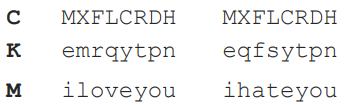
\includegraphics[scale=0.5]{one_time-pad.png}
\end{center}
\begin{flushleft}
It is an impractical method because:
\end{flushleft}
\begin{itemize}
  \item A 1GB file would need a 1GB key! 
  \item How are we transporting these keys? Or storing them? 
  \item If you ever reuse a key, the entire cipher is broken
\end{itemize}

\section{Modern Stream Ciphers}
\begin{itemize}
  \item Modern stream ciphers use an initial seed key to generate an infinite pseudorandom keystream 
  \item The message and keystream are usually combined using XOR - ⊕ - which is reversible if applied twice
  \item Common to seed an initial state using a key, then update this state for as long as needed
\end{itemize}

\begin{center}
  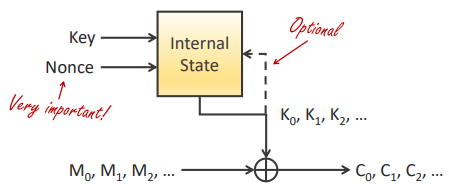
\includegraphics[scale=0.5]{modern_cyphers.png}
\end{center}

\subsection{ChaCha20}

\begin{center}
  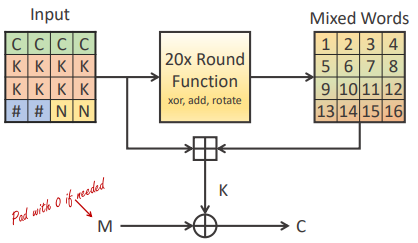
\includegraphics[scale=0.5]{chacha.png}
\end{center}
\begin{itemize}
  \item ChaCha performs 20 rounds: alternates Column and Diagonal Rounds, each round is 4 quarter rounds
  \item It's fast, because ChaCha20 is based on ARX (Addition-Rotation-XOR) which are \textbf{CPU friendly instruction}
\end{itemize}

\subsection{Advantages of Stream Ciphers}
\begin{itemize}
  \item Encrypting long continuous streams, possibly of unknown length 
  \item E.g. GSM mobile communications 
  \item Extremely \textbf{fast with a low memory footprint}, ideal for low-power devices 
  \item If designed well, can seek to any location in the steam. E.g. Streaming video with DRM
\end{itemize}

\subsection{Vulnerabilities}
\begin{itemize}
  \item Stream ciphers give us confidentiality, but not integrity 
  \item We must include another mechanism
\end{itemize}

\pagebreak
\section*{Reference section} \label{sec:reference}
\begin{description}
	\item[placeholder] \hfill \\
\end{description}
\end{document}
